\documentclass{article}
\usepackage[utf8]{inputenc}


\usepackage{tikz}
\usetikzlibrary{calc}

\begin{document}

\thispagestyle{empty}

\begin{figure}[h!]
		\centering
		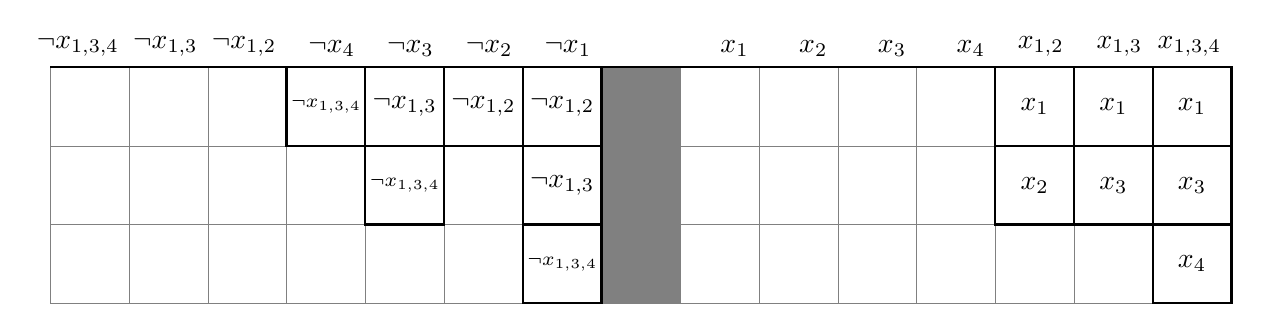
\begin{tikzpicture}
		%grid outline
		\draw[step=1cm,gray,very thin] (-7,0) grid (8,3);
		\fill[gray] (0,0) rectangle (1,3);
		
		%indexes
		\draw[thick] (-7,3) -- (-6,3) node[anchor=south east] {$\lnot x_{1,3,4}$};
		\draw[thick] (-6,3) -- (-5,3) node[anchor=south east] {$\lnot x_{1,3}$};
		\draw[thick] (-5,3) -- (-4,3) node[anchor=south east] {$\lnot x_{1,2}$};
		\draw[thick] (-4,3) -- (-3,3) node[anchor=south east] {$\lnot x_{4}$};
		\draw[thick] (-3,3) -- (-2,3) node[anchor=south east] {$\lnot x_{3}$};
		\draw[thick] (-2,3) -- (-1,3) node[anchor=south east] {$\lnot x_{2}$};
		\draw[thick] (-1,3) -- (0,3) node[anchor=south east] {$\lnot x_{1}$};
		\draw[thick] (0,3) -- (1,3);
		\draw[thick] (1,3) -- (2,3) node[anchor=south east] {$x_{1}$};
		\draw[thick] (2,3) -- (3,3) node[anchor=south east] {$x_{2}$};
		\draw[thick] (3,3) -- (4,3) node[anchor=south east] {$x_{3}$};
		\draw[thick] (4,3) -- (5,3) node[anchor=south east] {$x_{4}$};
		\draw[thick] (5,3) -- (6,3) node[anchor=south east] {$x_{1,2}$};
		\draw[thick] (6,3) -- (7,3) node[anchor=south east] {$x_{1,3}$};
		\draw[thick] (7,3) -- (8,3) node[anchor=south east] {$x_{1,3,4}$};
		
		%implications
		\draw[thick] (-4,3) rectangle (-3,2) node[pos=.5] {$\scriptstyle \lnot x_{1,3,4}$};
		
		\draw[thick] (-3,3) rectangle (-2,2) node[pos=.5] {$\lnot x_{1,3}$};
		\draw[thick] (-3,2) rectangle (-2,1) node[pos=.5] {$\scriptstyle \lnot x_{1,3,4}$};
		
		\draw[thick] (-2,3) rectangle (-1,2) node[pos=.5] {$\lnot x_{1,2}$};
		
		\draw[thick] (-1,3) rectangle (-0,2) node[pos=.5] {$\lnot x_{1,2}$};
		\draw[thick] (-1,2) rectangle (-0,1) node[pos=.5] {$\lnot x_{1,3}$};
		\draw[thick] (-1,1) rectangle (-0,0) node[pos=.5] {$\scriptstyle \lnot x_{1,3,4}$};
		
		\draw[thick] (5,3) rectangle (6,2) node[pos=.5] {$x_{1}$};
		\draw[thick] (5,2) rectangle (6,1) node[pos=.5] {$x_{2}$};
		
		\draw[thick] (6,3) rectangle (7,2) node[pos=.5] {$x_{1}$};
		\draw[thick] (6,2) rectangle (7,1) node[pos=.5] {$x_{3}$};
		
		\draw[thick] (7,3) rectangle (8,2) node[pos=.5] {$x_{1}$};
		\draw[thick] (7,2) rectangle (8,1) node[pos=.5] {$x_{3}$};
		\draw[thick] (7,1) rectangle (8,0) node[pos=.5] {$x_{4}$};
		\end{tikzpicture}
		\caption{Lists of binary implications.}
		\label{fig:binary_implications}
	\end{figure}

\end{document}
